\begin{auf}
    614
\end{auf}
Elektronen durchlaufen in einer Elektronenstrahlröhre zunächst eine Beschleunigungsspannung von $U=15kV$ und werden anschließend durch ein senkrecht zum Elektronenstrahl angeordnetes homogenes Magnetfeld von $B=8\cdot10^{-3}T$ abgelenkt. Die Anfangsgeschwindigkeit der Elektronen sei null, ihre spezifische Ladung beträgt $\frac{e}{m_e}=1.76\cdot10^{11}\frac{C}{kg}$.
\begin{enumerate}
    \item[a] Mit welcher Geschwindigkeit $v$ treten die Elektronen ins Magnetfeld ein?
    \item[b] Wie groß ist der Krümmungsradius $r$ der Bahn im Magnetfeld?
    \item[c] Mit welcher Geschwindigkeit $v_1$ treffen die Elektronen auf dem Leuchtschirm auf?
\end{enumerate}
\begin{figure}[h]
    \centering
    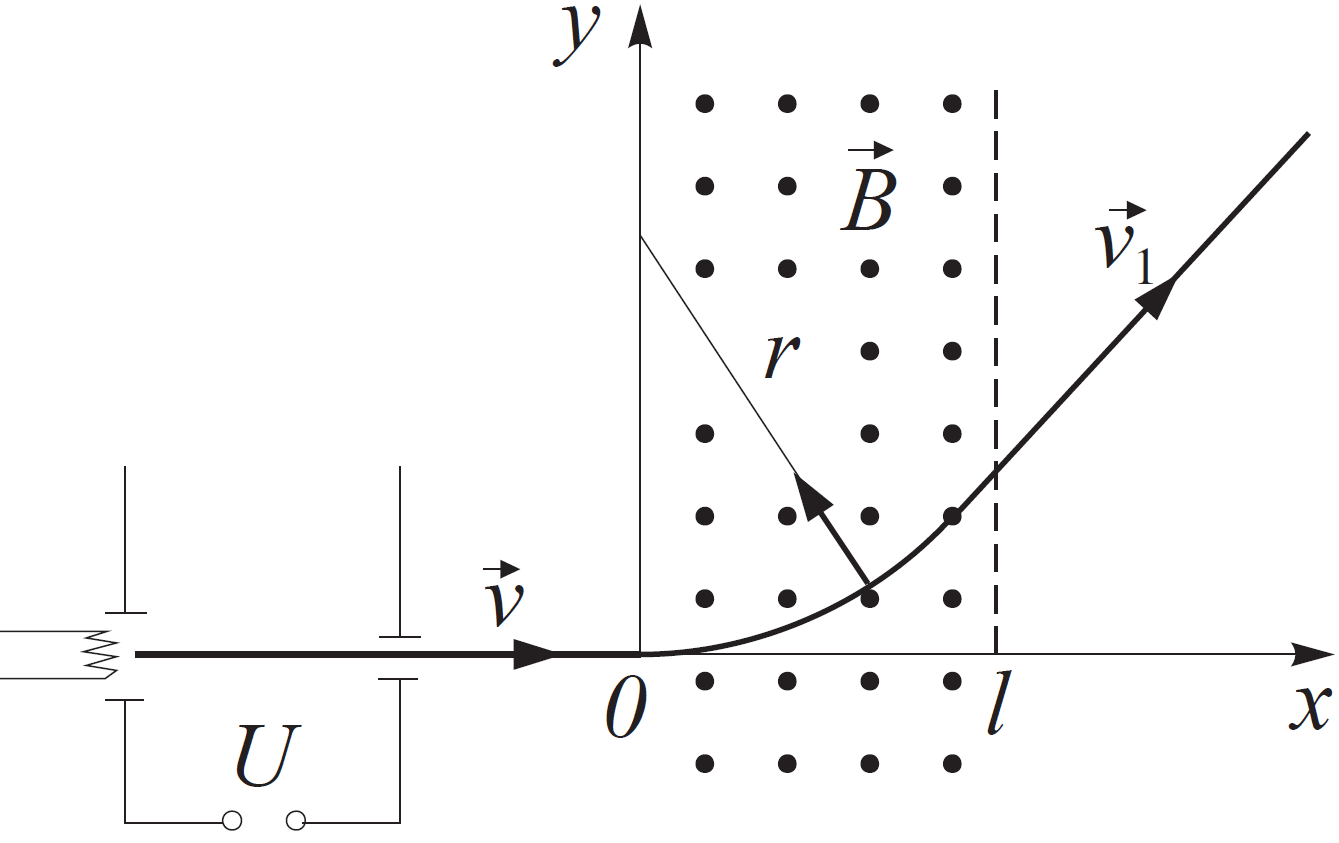
\includegraphics[width=0.7\linewidth]{images/614_0.png}
    \caption{Versuchsaufbau Aufgabe 614}
\end{figure}